Bioptim was used to optimize joint kinematics and kinetics that maximize vertical jump height.
Using a joint torque driven model, we simulated only the push-off phase that was divided into two phases:
first phase with two contact points (heel and toe),
and second phase with one contact (toe). Phase times were bounded: [0.2, 1.0] and [0.05, 1.0].

The actuators bounds were modeled using a custom nonlinear constraint to account for the torque-angle-angular
velocity relationship using the gauss3p function of biorbd based on predetermined factors
(\ref{fig:graph_force_vitesse_longueur}).

The first term of the objective function corresponds to the jump height.
The second term of the objective function corresponds to the time variation.
It allows the solver to get the best jump with the shortest time.

Using ipopt solver, the problem was first launched using the BFGS hessian approximation feature for 200 iterations.
Then if the maximum number of iterations is reached,
the solution was re-optimized with a exact hessian computations with up to 1000 iterations using a warm start.

The height of the jump is 1,35m.
The strategy used is XXX with a proximo-distal shift of the joints (hip, knee then ankle) highlighted by the
activation of the hip, then the knee and finally the ankle.

\begin{figure*}[t!]
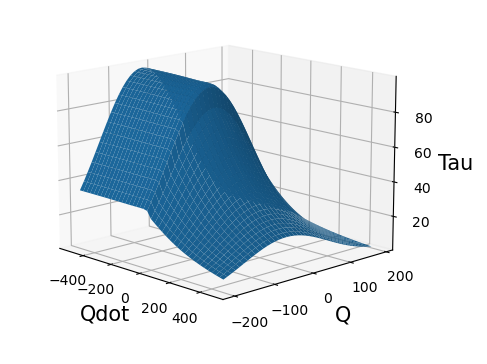
\includegraphics[width=\textwidth/2]{figures/graph_force_vitesse_longueur.png}\\
\caption{Surface getting torque range from q and qdot}
\label{fig:graph_force_vitesse_longueur}
\end{figure*}
